\documentclass{article}

\usepackage[utf8]{inputenc}
\usepackage[T1]{fontenc}      
\usepackage[francais]{babel}
\usepackage{chemist}
\usepackage{chemfig} 
\usepackage{lewis}
\usepackage[top=2.5cm,bottom=2.5cm,right=2.5cm,left=2.5cm]{geometry}
\usepackage[squaren, Gray]{SIunits}
\usepackage{url}

\newcommand\chemfigc[1]{
\vspace{0.5cm}
\begin{center}\chemfig{#1}\end{center}
\vspace{0.5cm}}

\title{Projet 3 - Rapport de tâche 1}
\author{\textbf{Groupe 124.3}
\\
\textsc{Frenyo} P\'eter (6266-12-00)\\
\textsc{Gillain} Nathan (7879-12-00)\\
\textsc{Lamine} Guillaume (7109-13-00)\\
\textsc{Piraux} Pauline (2520-13-00)\\
\textsc{Paris} Antoine (3158-13-00)\\
\textsc{Quiriny} Simon (4235-13-00)\\
\textsc{Schrurs} Sébastien (7978-13-00)}
\date{\today} 
\begin{document}

\maketitle

\section{Calcul du flux des réactifs}

\paragraph{Hypothèse}
Lors du calcul de ces flux, nous avons utilisé l'hypothèse que tous les réactifs sont 
consommés par le réacteur.

\paragraph{Calculs}
L'équation de la réaction de production de l'ammoniac par le procédé \textsc{Haber-Bosch} est donnée par :

	\begin{chemmath}
			\frac{1}{2}N_2(g) + \frac{3}{2}H_2(g) \longrightarrow NH_3(g) + \Delta H
 	\end{chemmath}
	
En sachant que l'on cherche à produire \unit{1000}{\ton} de \chemform{NH_3} par jour, 
on calcule assez facilement le flux de \chemform{N_2} (les détails de calculs ont été omis
dans ce rapport)

	$$m_{N_2} = \unit{823.5}{\ton\per\dday}$$

et le flux de \chemform{H_2}

	$$m_{H_2} = \unit{176.4}{\ton\per\dday}.$$

\section{Calcul du débit d'eau nécessaire pour refroidir le réactif}
\paragraph{Hypothèses}
\begin{itemize}
	\item Les capacités calorifiques ne dépendent pas de la température ;
	\item La pression dans le réacteur est constante et vaut \unit{10^5}{\pascal}.
\end{itemize}

\paragraph{Première méthode : on considère les capacités calorifiques constantes}
Pour la réaction donnée dans la section précédente, on a $\Delta H(\unit{298.15}{\kelvin})
 = \unit{-46 \cdot 10^3}{\joule}$ pour une mole de \chemform{NH_3(g)} produite \cite{atkins}.
Comme la réaction a lieu à \unit{500}{\celsius} (c'est à dire \unit{773.15}{\kelvin}), il
va falloir calculer $\Delta H(\unit{773.15}{\kelvin})$. Pour cela, nous avons besoin
des capacités calorifiques moyenne à pression constante de chacun des réactifs et des produits
de la réaction. Nous trouvons ces données dans une table \cite{atkins}.

	$$
	\left\{
		\begin{array}{rl}
			C_{p_{NH_3(g)}} &= \unit{37}{\joule\per\mole\kelvin}\\
			C_{p_{H_2(g)}} 	&= \unit{28.836}{\joule\per\mole\kelvin}\\
			C_{p_{N_2(g)}} 	&= \unit{29.124}{\joule\per\mole\kelvin}
		\end{array}
	\right
	$$

On a donc :

$$\Delta H(\unit{773.15}{\kelvin}) = \Delta H(\unit{298.15}{\kelvin})
+ \int_{298.15}^{773.15} C_{p_{NH_3(g)}} dT - \frac{1}{2}\int_{298.15}^{773.15} C_{p_{N_2(g)}} dT
- \frac{3}{2} \int_{298.15}^{773.15} C_{p_{H_2(g)}} dT = \unit{-5.5887 \cdot 10^4}{\joule\per\mole}$$

Pour la quantité de \chemform{NH_3} à produire par jour (à savoir $\unit{58.83 \cdot 10^6}{\mole}$),
la quantité de chaleur produite est donc :

$$q = \Delta H(\unit{773.15}{\kelvin}) \cdot n_{NH_3} = \unit{-3.28786 \cdot 10^{12}}{\joule}$$

En connaissant la capacité calorifique de l'eau $C_{H_2O(g)} = \unit{4185.5}{\joule\per\kilo\gram\kelvin}$ \cite{atkins}et en égalant
$q$ à $m_{H_2O} \cdot C_{H_2O(g)} \cdot \Delta T$ avec $\Delta T = 90 - 25 = \unit{65}{\kelvin}$, on trouve un
flux d'eau égal à

$$m_{H_2O} = \unit{1.2085 \cdot 10^7}{\kilo\gram\per\dday} \Rightarrow V_{H_2O} \approx \unit{1.2085 \cdot 10^7}{\liter\per\dday} 
= \unit{139.8}{\liter\per\second}$$

\paragraph{Deuxième méthode : les capacités calorifiques dépendent de la température}
On peut être plus précis en utilisant les capacités calorifiques suivantes \cite{hc-table} :

	$$
	\left\{
		\begin{array}{rl}
			C_{p_{NH_3(g)}}(T) &= \unit{31.81 + (15.48 \cdot 10^{-3})T + (5.86 \cdot 10^{-6})T^2}{\joule\per\mole\kelvin}\\
			C_{p_{H_2(g)}}(T) 	&= \unit{29.30 - (0.84 \cdot 10^{-3})T + (2.09 \cdot 10^{-6})T^2}{\joule\per\mole\kelvin}\\
			C_{p_{N_2(g)}}(T) 	&= \unit{27.62 + (4.19 \cdot 10^{-3})T}{\joule\per\mole\kelvin}
		\end{array}
	\right
	$$

En refaisant le calcul ci-dessus en tenant compte de la variation des capacités calorifiques en fonction
de la température, nous obtenons un débit un peu inférieur de \unit{135.662}{\liter\per\second}. On remarque
que l'approximation faite ci-dessus n'est pas si mauvaise que ça. Nous vous épargons ici
les détails de calculs (que nous avons réalisé avec \textsc{Matlab}).

\section{Sources des réactifs}
	\subsection{Sources de diazote}
	\subsubsection{Procédé cryogénique}
	Ce procédé se base sur la séparation des différents constituants de l'air en fonction de leur température 
	d'ébullition (l'oxygène \chemform{O_2} se condense avant le diazote \chemform{N_2}).
	L'air est purifié jusqu'à liquéfaction et les différents constituants sont séparés dans une colonne de 
	rectification par distillation fractionnée. Cette méthode permet d'avoir du diazote \chemform{N_2} pur 
	à \numprint{99,99}\%. Cette méthode est efficace pour une consommation au-delà de $\unit{200}{\meter\cubed\per\hour}$ \cite{scf}. 

	\subsubsection{Perméation gazeuse}
	Ce procédé utilise les différentes vitesses d'effusion des molécules de gaz à travers une membrane. 
	L'\chemform{O_2}, \chemform{H_2O} et le \chemform{CO_2} s'effusent plus rapidement que le \chemform{N_2}.
	Cette méthode nous permet d'obtenir du \chemform{N_2} sec pur à \numprint{95-99}. Ce procédé s'utilise pour des 
	débits forts variables ($\unit{3-1000}{\meter\cubed\per\hour}$) \cite{scf}.

	\subsubsection{Méthode de Ramsay}
	
	\begin{chemmath}
			NaNO_2(aq) + NH_4Cl(aq) \longrightarrow NaCl(aq) + 2 H_2O(l) + N_2(g)
	\end{chemmath}
	
	On chauffe le mélange de \chemform{NaNO_2} et \chemform{NH_4Cl} pour obtenir le \chemform{N_2} sous forme gazeuse.
	Un désavantage de cette méthode par rapport aux 2 premières est qu'il faut acheter les réactifs. De plus, il faut utiliser de l'énergie pour chauffer la réaction \cite{wiki-n2}.

	\subsection{Sources de dihydrogène}
		\subsubsection{Vaporeformage de méthane}
		2 réactions sont utilisées pour ce procédé \cite{afhypac} :
		
		\begin{chemmath} 
			CH_4 + H_2O \longleftrightarrow CO + 3H_2
		\end{chemmath}
		
		\begin{chemmath}
			CO + H_2O \longleftrightarrow CO_2 + H_2
		\end{chemmath}
		
		L'équation bilan obtenue est la suivante :
		
		\begin{chemmath}
			CH_4 + 2H_2O \longleftrightarrow CO_2 + 4 H_2
		\end{chemmath}
		
			Cette réaction nécessite un catalyseur : le nickel. Le rendement varie entre $40-45\%$. Le problème de cette 
			méthode est qu'elle rejette une grande quantité de \chemform{CO_2}, gaz à effet de serre \cite{wiki-h2}.
			
		\subsubsection{Oxydation partielle d'hydrocarbure}
		\begin{chemmath}
			C_nH_m + \frac{n}{2} O_2 + \frac{3,76n}{2} N_2 \longrightarrow \frac{m}{2} H_2 + n CO + \frac{3,76n}{2} N_2
		\end{chemmath}
		L'air est comburant pour cette réaction, qui a besoin d'être catalysée. Son caractère exothermique aide à la catalyse. 
		L'inconvénient de cette méthode est son faible rendement \cite{wiki-h2}.

		\subsubsection{Electrolyse}
		Réaction à l'anode : 
		
		\begin{chemmath}
			2H_2O(l) \longrightarrow O_2(g) + 4 H^+(aq) + 4e^-
		\end{chemmath}
		
		Réaction à la cathode :
		
		\begin{chemmath}
			4H_2O(l) + 4e^- \longrightarrow 2H_2O(g) + 4OH^-(aq)
		\end{chemmath}
		
		L'équation bilan obtenue est la suivante :
		
		\begin{chemmath}
			2H_2O(l) \longrightarrow 2H_2(g) + O_2(g)
		\end{chemmath}
		
	La réaction nécessite une grande quantité d'électricité. L'eau, quant à elle, est présente en quantité illimitée 
	et est peu coûteuse. En pratique, cette méthode est très peu utilisée \cite{wiki-h2}.
	
	\section{Flow-sheet}
	La première ébauche de notre flow-sheet se trouve à la figure \ref{flow-sheet}.
	
	\begin{figure}[ht!]
		\centering
		\rotatebox{90}{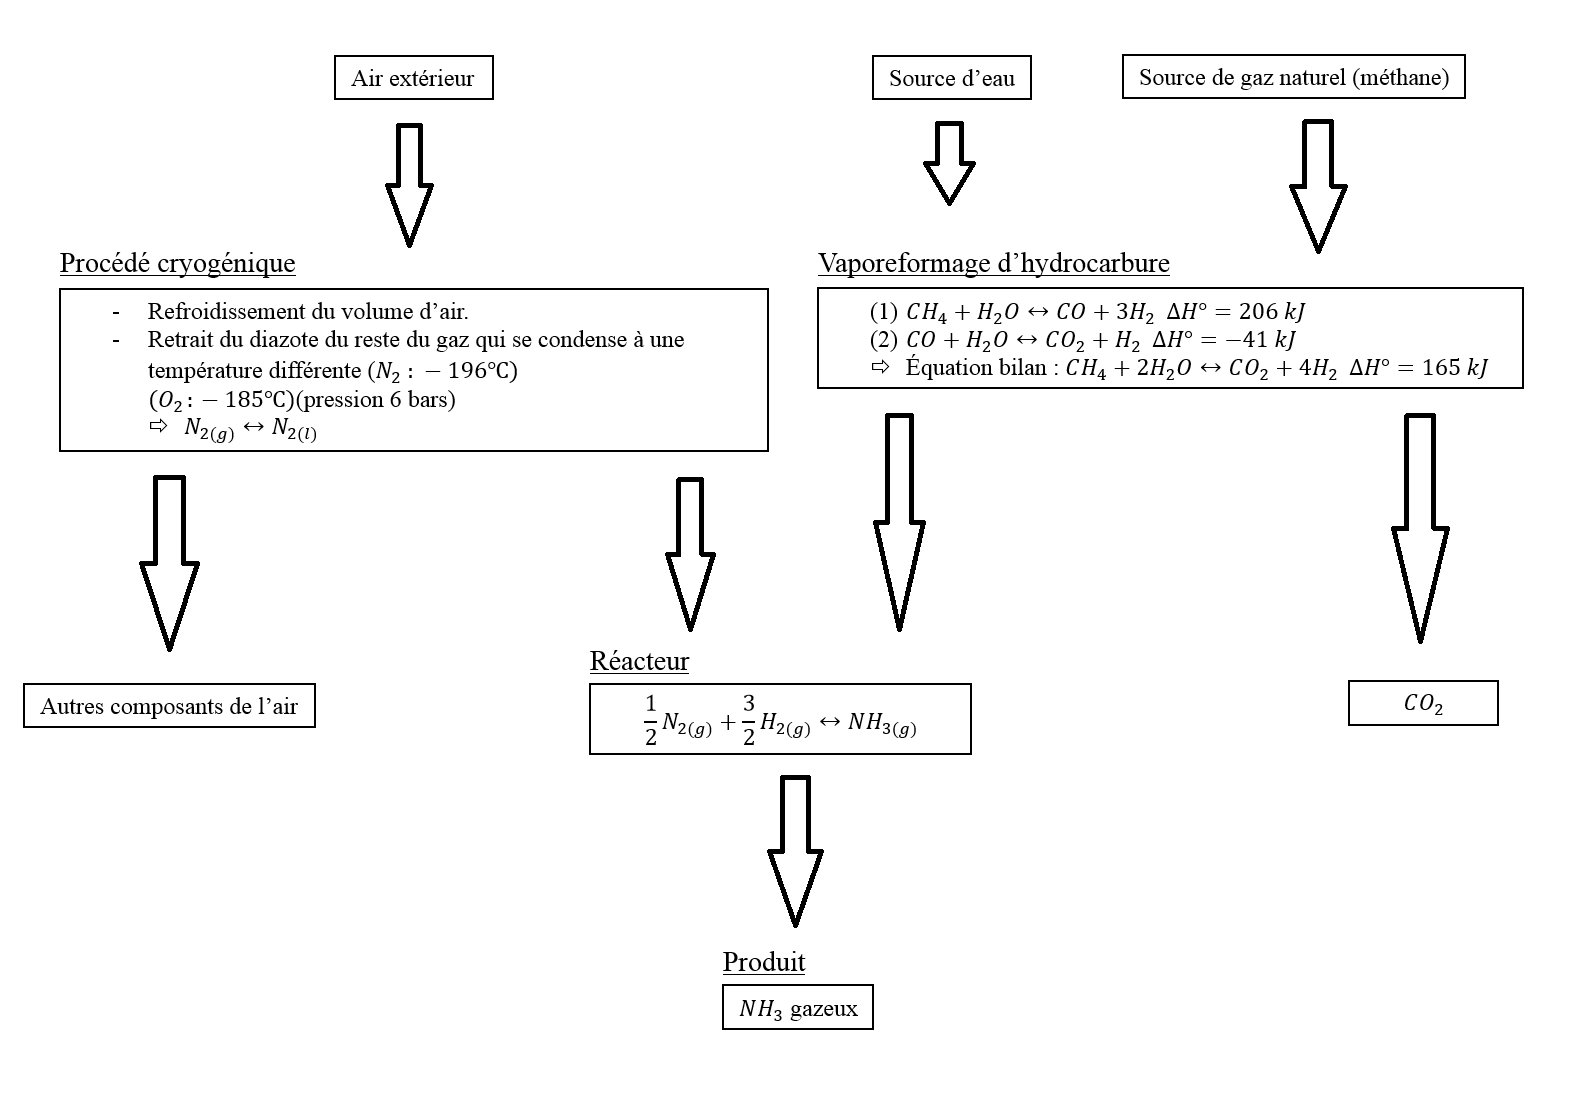
\includegraphics[scale=0.50]{flow-sheet.png}}
		\caption{Première ébauche de notre flow-sheet.}
		\label{flow-sheet}
	\end{figure}

\section{Bilan de mati�re}
% To do

\section{Equilibre du reformage primaire}
% To do

\section{Bilan d'�nergie}
% To do

\section{Outil de gestion}
% To do

\section{Calcul du nombre de tuyaux}
% To do

\bibliography{source-tache1}
\bibliographystyle{plain}
\nocite{*}
	
\end{document}
